\documentclass{acm_proc_article-sp}


\usepackage{gregmath}
\usepackage{url}
\usepackage{amsmath}
\usepackage{amssymb}
\usepackage{graphicx}
\usepackage{color}
\usepackage{subfigure}
\usepackage[colorlinks=true, citecolor=blue]{hyperref}
\usepackage{algorithm}
\usepackage{algorithmic}
\usepackage{framed}

\graphicspath{{./pdf/}}

\begin{document}

\title{Feature Subset Selection for Inferring Relative\\Importance of Taxonomy\titlenote{Permission to make digital or hard copies of part or all of this work for personal or classroom use is granted without fee provided that copies are not made or distributed for profit or commercial advantage and that copies bear this notice and the full citation on the first page. Copyrights for third-party components of this work must be honored. For all other uses, contact the Owner/Author.Copyright is held by the owner/author(s).\\ 
BCB '14 , Sep 20-23 2014, Newport Beach, CA, USA
ACM 978-1-4503-2894-4/14/09. \\
\url{http://dx.doi.org/10.1145/2649387.2660824}}
}

\numberofauthors{2} 
\author{
\alignauthor
Gregory Ditzler\titlenote{Corresponding author.}\\
       \affaddr{Drexel University}\\
       \affaddr{Dept. of Electrical \& Computer Engineering}\\
       \affaddr{Philadelphia, PA 19104 USA}\\
       \email{gregory.ditzler@gmail.com}
\alignauthor 
Gail Rosen\\
       \affaddr{Drexel University}\\
       \affaddr{Dept. of Electrical \& Computer Engineering}\\
       \affaddr{Philadelphia, PA 19104 USA}\\
       \email{gailr@ece.drexel.edu}
}


%\date{30 July 1999}

\maketitle
\begin{abstract}

Examining the bacterial or functional differences between multiple habitats/populations/phenotypes plays an important role in making inferences about the roles that the taxonomy and functional profiles can take on in microbial ecology. It is therefore important to the field of comparative metagenomics, using $\alpha$- \& $\beta$-diversity, that methods or algorithms can detect the importance of particular subsets of variables that best differentiate the multiple phenotypes in the data. Given todays genomic {\em data deluge} efficient methods that can carry out these inferences cannot be understated enough. We assume observations are collected from a multitude of different environments (e.g., males vs. females, control vs. stimulus, etc.), and each observation is comprised of hundreds or thousands of different taxa/functional features (i.e., 16S or whole genome shotgun). Our goal in this work is to examine the role, assumptions, and inferences that feature subset selection can provide the field of microbial ecology and comparative metagenomics. 
Specifically we examine feature subset selection algorithms using embedded and filter approaches to infer taxa importance on data collected from the human gut microbiome 
We compare several widely adopted approaches from machine learning including greedy algorithms and $l_1$ regularization methods, as well as some software tools provided with QIIME, on data collected from the American Gut Project and other canonical studies of the human gut microbiome. 
We find that there are very few OTUs that carry information in regards to predicting the sex of a gut sample, and that {\em Bacteroidetes} is quite frequently found in the top ranked OTUs. 

\end{abstract}

% A category with the (minimum) three required fields
%\category{H.4}{Information Systems Applications}{Miscellaneous}
%A category including the fourth, optional \footnote{?}ield follows...
%\category{D.2.8}{Software Engineering}{Metrics}[complexity measures, performance measures]

%\terms{Theory}

%\keywords{Information-Theoretic Feature Subset Selection, Data Mining, Taxonomic Discovery} 

\section{Introduction}

The amount of data being generated by fields in life science is almost unfathomable to what what was being  generated just a decade ago. The field of genomics has observed data growth rates as well \cite{BigDataBook}, and the cost of collecting such data is more rapid than Moore's law could have predicted\footnote{Refer to \url{http://www.genome.gov/sequencingcosts/}}. Given this {\em data deluge} in genomics, it is apparent to the success of the field that comparative analysis tools of today are capable of scaling to the data of tomorrow, and still give researchers meaningful interpretations of their data. The engineering and computational intelligence community has already begun to perform translational research that can benefit the many fields within the life sciences \cite{Vidyasagar2012CSM}, and specifically, the field of machine learning can provide extremely useful information to researchers in the life sciences. 


In this work, we specifically focus on areas related to comparative metegenomics (and 16S analysis). Specifically, we assume that the raw sequences from the environmental samples have already been classified into operational taxonomic units (OTUs), or functions. The raw OTU\footnote{We use OTU from this point forward. The analysis for working with functional profiles is identical in our work, therefore, we use OTUs for brevity.} counts are stored in a  matrix $\Xbf \in \Nbb_{+}^{K \times N}$, where $\Nbb_{+}$ is the set of positive natural numbers, $K$ is the number of OTU clusters, and $N$ is the number of samples collected. The $N$ samples contain a significant amount of {\em metadata} describing the sample, which is were we obtain phenotypes describing the sample. While there may be quite a few pieces of metadata, we shall only focus on one piece of metadata at a time. For example, a sample may contain the sex, age, and height of the person from where a sample was collected, and the analysis would only use {\em one} of those fields. That is we could use $\Xbf$ to build a predictive model of sex. Both the data matrix and metadata can be found for hundreds of datasets though pioneering projects such as MG-RAST \cite{Meyer2008BMCBio}, KBase \cite{KBase}, the Human Microbiome Project \cite{HMP2009}, and the Earth Microbiome Project \cite{Gilbert2010SGS}.  

The data matrix $\Xbf$ is comprised of many OTUs (e.g., the data from the American Gut Project has 25k+), although, as we shall show, many of them may carry little information about differentiating  something such as the sex of the sample. Therefore, we use feature subset selection algorithms to detect the number of relevant features, or OTUs, that best differentiate the phenotypes. The field of feature subset selection can provide these types of insights into the importance of OTUs, and recent efforts have begun to scale these methods to massive datasets to keep up with todays data needs \cite{Zhia2014CIM, Liu2010FSW}. We also show how one recent subset selection method for big data can be useful for determining taxa importance via a statistical hypothesis test. 

This manuscript is organized as follows: section \ref{sec:rwork} covers the background and related works to elements of feature subset selection and how it relates to works in comparative metagenomics. Section \ref{sec:methods} describes the methods used to carry out the experiments in section \ref{sec:exp}. Finally, section \ref{sec:conc} provides some concluding remarks on the results and directions for future research. 



\section{Related Works}
\label{sec:rwork}

The core of this work lies in that of supervised learning. That is learning a mapping from an input space $\Xcal$ (e.g., OTUS) to an outcome (e.g., health status), which gives us a strong motivation to evaluate the features that best represent the problem prior to learning a predicting model, such as a SVM or $k$-NN classifier. Several recent works have begun to examine the role of supervised learning in the microbiome \cite{Knights2011FEMS, Fierer2010NAS},  and multi-class learning \cite{Lui2011Bio}. In these works, feature selection has been considered from an embedded perspective, while our previous work sought to use an information-theoretic perspective \cite{Garbarine2011CBC, Ditzler2012ICASSP, Ditzler2012GENSIPS}. In this work we continue to evaluate feature selection using embedded and information-theoretic methods, and we evaluate the amount of predictive information in the differentiation between male and females' OTU abundance profiles. 


\section{Methods}
\label{sec:methods}


Feature subset selection approaches typically fall one of three categories: {\em wrapper}, {\em embedded} and {\em filter} methods. Wrapper based algorithms use a score computed from cross validation performance of a chosen classifier to search the subspace of features that will yield a subset of features that minimize the score. Unfortunately these methods are overly complex and do not scale to big data even with ``more efficient'' implementations. Therefore, we do not examine wrapper based algorithms   in this work. 

Embedded methods jointly optimize the  classifier's parameters and feature selector simultaneously \cite{Guyon2006Book, Guyon2003JMLR}. The difference between embedded and wrapper based approaches, is that the feature selection for embedded methods is built into the objective function being optimized, which is not the situation for a wrapper method. Filter-based methods decouple the feature selection objective from classification by scoring feature independently from an error function. Hence, filter are typically very fast compared to wrappers or embedded approaches. In this work, we examine the use of filter-based approaches using information theory and embedded methods that induced a sparse solution using a minimization of the $l_1$ norm of a parameter vector. 


\subsection{Greedy Algorithms, Information Theory \& NPFS}
\label{sec:greed}
One of the fundamental quantities in information theory that has been widely adopted for feature subset selection with filters is {\em mutual information}, which is given by:
\begin{align}
  \textsf{I}(X;Y) = \sum_{y\in\Ycal}\sum_{x\in\Xcal} p_{X,Y}(x,y) \log \frac{p_X(x)\,p_Y(y)}{p_{X,Y}(x,y)}
  \label{eq:mi}
\end{align}
where $p_X(x)$ is the marginal distribution over the random variable $X$ and $p_{X,Y}(x,y)$ is the joint probability distribution over $X$ and $Y$. Hence, mutual information is the scoring function for determining the set of features $\Fcal$ that carry the most information about an outcome $Y$. A simple algorithm for feature selection with a filter is the {\sl greedy forward selection search} which seeks to maximize feature scoring function $\Jcal$, which is shown in Figure \ref{fig:greedy}. The initializes the relevant feature set $\Fcal$ to be empty. Then for $k$ iterations an objective function $\Jcal$ is maximized, and the feature that maximizes the expression is added to the relevant feature set, $\Fcal$, and removed from the feature set, $\Xcal$. Simply using mutual information as the objective function is a fast way for microbial ecologists to examine the relative importance of taxa in a study collected from environmental samples. Though simply using mutual information will not capture inter-feature dependencies. Using other objective functions, such as joint mutual information \cite{Yang1999NIPS}, captures some of the inter-feature dependencies.


\begin{figure}
  \begin{framed}
    {\bf Input}: Collection of features $\Xcal:=\{X_i: i \in[K]\}$, scoring function $\Jcal$, and phenotype variables $Y$. \\
    {\bf Initialize}: $\Fcal = \varnothing$ \\
    {\bf while} $|\Fcal| < k$ {\bf do}
    \vspace{-.5em}
    \begin{mitemize}
      \item Compute next best feature
        \begin{align}
          X^* = \arg\max_{X' \in \Xcal} \Jcal(X',Y,\Fcal)
        \end{align}
      \item $\Fcal \leftarrow \Fcal \cup X^*$
      \item $\Xcal \leftarrow \Xcal \backslash X^*$
    \end{mitemize}
    \vspace{-.5em}
    {\bf end while}
  \end{framed}
  \caption{Pseudo code for search selecting features using a greedy algorithm that attempts to maximize $\Jcal$. }
  \label{fig:greedy}
\end{figure}

Our recent work includes the development of the Neyman-Pearson Feature Selection (NPFS), which automatically detects the relevant features in a dataset using a generic scoring function \cite{Ditzler2014TNNLS}. Furthermore, NPFS is highly parallelizable, which allows it to be quite effective for very large datasets. NPFS works by mapping out random samples of the original dataset to a scoring function which makes a prediction on which features are relevant. All of the sub-datasets have the same number of features selected then in a reduction phase NPFS applied the Neyman-Pearson test to detect feature importance. In this setting, NPFS can detect the number of important OTUs simply by guessing $k$ in Figure \ref{fig:greedy} for the scoring function and letting the hypothesis detect features that appear to be more important. 

\subsection{Regularization for Subset Selection}
Section \ref{sec:greed} presented a greedy algorithm and tools from information theory that can be used to select features that are deemed important by the scoring function. Now we present feature selection from an embedded perspective. Let $\ybf$ be a vector in $\{\pm 1\}^{N}$ containing a binary outcome (e.g., control or stimulus) and $\Xbf$ be abundance matrix. Predictions are made on $\ybf$ with $\Xbf^\T\theta$, where $\theta \in \Rbb^K$. If many of the entries of $\theta$ were zero then we could view the inner product of $\theta$ with $\Xbf$ as a form of feature selection. To encourage sparsity in $\theta$'s solution, Tibshirani presented lasso, which adds a penalty to the $l_1$-norm of $\theta$ \cite{Tibshirani1996JRSS}. Formally, lasso is given by:
\begin{align}
  \theta^* = \arg\max_{\theta\in\Theta} \frac{1}{2N} \| \ybf - \Xbf^\T\theta \|_2^2 + \lambda \|\theta\|_1
\end{align}
where $\lambda > 0$, and $\|\cdot\|_1$ and $\|\cdot\|_2$ are the $l_1$- and $l_2$-norms, respectively. For lasso to be effective at feature selection, it is assumed that $K \gg N$, which is typically an acceptable assumption with 16S and metagenimic data because there are typically only a few samples and a large number of features. The elastic-net was developed to avoid lasso selecting all features when  $K \gg N$ is not met (see \cite{Zou2005JRSS}). The objective function of the elastic net is given by:
\begin{align}
  \theta^* = \arg\max_{\theta\in\Theta} \frac{1}{2N} \| \ybf - \Xbf^\T\theta \|_2^2 + \lambda_1 \|\theta\|_1 + \frac{\lambda_2}{2} \|\theta\|_2^2
\end{align}

\subsection{Normalization and Scaling $\Xbf$}

In this work we do not use the raw OTU abundance abundance rather we use a scaled version of the relative abundance, and Su et al. demonstrate that using normalizations can improve the interpretability of the analysis \cite{Su2012TCBB}; however, Su et al. did not evaluate normalization's impact on feature selection. We normalize the columns of $\Xbf$ to produce a relative abundance matrix, $\Xbf'$, which is then used for feature subset selection. We scale $\Xbf'$ by a factor $\gamma$ to avoid numerical issues. 



\section{Experimental Results}
\label{sec:exp}


We evaluated several publicly available software tools for feature subset selection -- some of which are  implemented for biological data formats (see ${\dagger}$). Below is a summary of the algorithms tested: 
\begin{mitemize}
\item {\sf Fizzy}$^{\dagger}$: Fizzy is a feature subset selection tool for biological data formats that is built on  top of Brown et al.'s FEAST Toolbox \cite{Brown2012JMLR}. The experiments in this section use mutual information maximization (MIM) \cite{Lewis1992MIM}, unless otherwise stated. MIM uses \eqref{eq:mi} as the objective function in Figure \ref{fig:greedy}. The Fizzy libraries were modified to directly output the mutual information scores (see GitHub for more details.)
\item {\sf NPFS}$^{\dagger}$: NPFS detects feature importance given a base subset selection algorithm \cite{Ditzler2014TNNLS}. We use command line tool for NPFS and use MIM as the base subset selection algorithm with 500 bootstraps.  
\item {\sf Lasso}: Lasso is implemented in the Scikit-Learn machine learning package for Python \cite{scikit-learn}. We set $\lambda=1$ and the maximum number of iterations to 1000. 
\item {\sf Elastic-Net}: The elastic net is implemented in the Scikit-Learn machine learning package for Python \cite{scikit-learn}. We give equal weight to the penalization of the $l_1$ and $l_2$ norms, and the maximum number of iterations to 1000.
\item {\sf Random Forest}$^{\dagger}$: The random forest was implemented using QIIME's {\tt supervised\_learning.py} function  \cite{Caporaso2010NM}. The ensemble is generated with 500 trees using the out-of-bag error estimate. The random forest can rank features based on the average drop in accuracy if the feature is omitted from the dataset. 
\end{mitemize}


We have released code and data required reproduce the tabular results and figures. This supplemental information is available at \url{https://github.com/gditzler/BigLS2014-Code}. Furthermore, the data from the American Gut Project was obtained from \url{https://github.com/biocore/American-Gut}, and Caporaso et al.'s microbiome study was obtained from the Earth Microbiome Project (study identifier 550) \cite{Caporaso2011GB, Gilbert2010SGS}. Our primary motivation for selecting benchmark datasets collected from the human gut was because it has been well studied, and becoming increasingly more understood \cite{Caporaso2011GB, Arumugam2011Nat, Koenig2010NAS, Turnbaugh2009Nature, MetaHit, Yatsunenko2012Nature}. Thus, we can refer back to existing literature to verify that our results go along with our intuition. The  metadata values for the sex of the sample is used as the phenotype (i.e., class labels). The data from the American Gut Project contains 469 samples (231/238 male/females), and 25703 OTUs. The Caporaso data contains 467 samples (336/131 males/females) with 16703 OTUs.


\subsection{On the Information in Taxonomy}
In our first experiment, we evaluate the amount of mutual information that can be found in the OTU abundance table from the American Gut Project. To examine this, bootstrap samples are drawn from the entire data and the mutual information is computed. For clarity, only the top 2000 OTUs mutual information are reported in Figure \ref{fig:mi boots}. Note that we have sorted the $x$-axis according to the mutual information level. The grey line indicates the MI from one of the bootstrap trials and the black line is the average from mutual information.  

One of the primary observations to make is that the vast majority of the OTUs have very little information shared with the sex phenotype. In fact, we can infer that there are only -- approximately -- OTUs that are somewhat informative for differentiating the sex of a sample. NPFS detects 73 OTUs as being important, and 30 of them are unique, which reconfirms that there are very few informative features for differentiating the sex of the sample. 


\begin{figure}
  \centering
  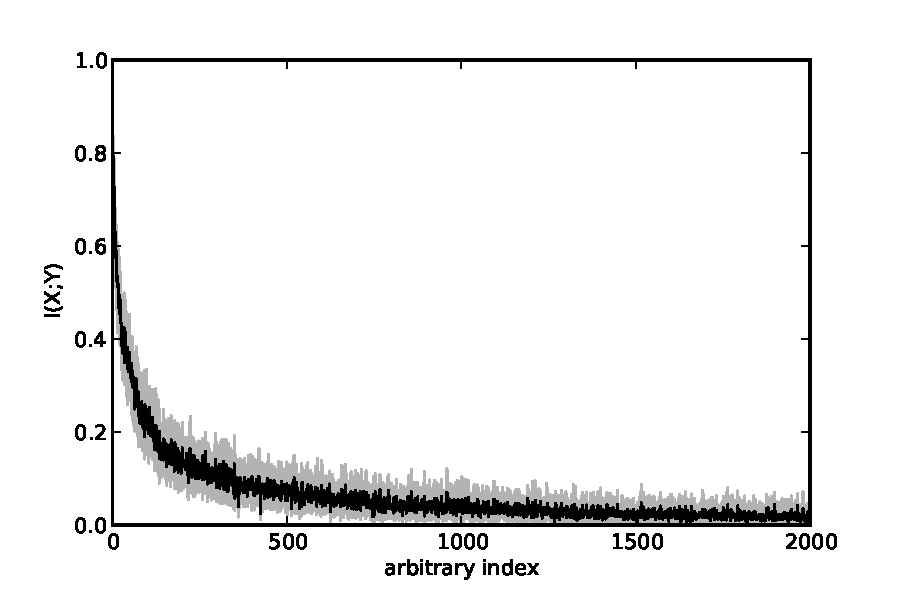
\includegraphics[width=.45\textwidth]{ag-mf-mi-bootstraps.pdf}
  \caption{Mutual information shared between the taxa and \texttt{sex} phenotype for data collected from the American Gut Project. The mutual information is calculated over 50 bootstraps of the top ranked 2000 of 25k+ taxa. }
  \label{fig:mi boots}
\end{figure}

Figure \ref{fig:mi} shows another view of the mutual information in the American Gut Data; however, in this figure the mutual information is calculated as $\textsf{I}(X_i;X_j)$, which ignores the phenotype. Again, we find relative few of the relevant features (as determined by $\textsf{I}(X;Y)$), share information with other top ranked OTUs as determined by MIM. Similar observations can be made when lasso is evaluated on this data. Figure \ref{fig:lasso coeff} shows the weights of lasso ($\theta$) with the largest magnitude, and again the observation is that there are relatively few features (<100) that appear to be informative for predicting the sex phenotype. Figure \ref{fig:lasso coeff} was generated with $\lambda=1$. Figure \ref{fig:lasso mse} shows that there is relatively little variation in lasso's mean squared error (MSE) when evaluated as a function of $\lambda$. Elastic nets provide nearly identical results for data from American Gut Project, therefore, we have omitted the results to avoid  redundancy. 

\begin{figure*}
  \centering
  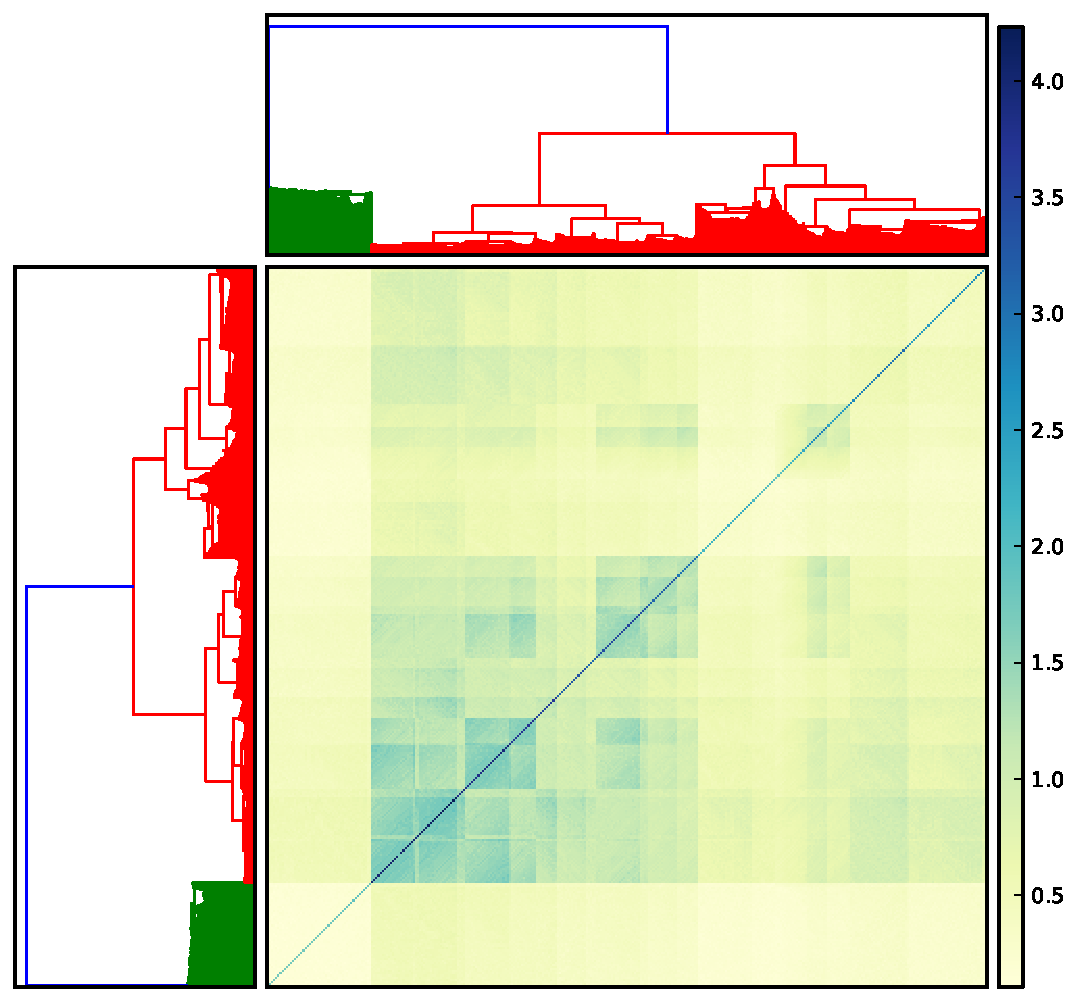
\includegraphics[width=.6\textwidth]{ag-t1000-mutual-information.pdf}
  \caption{Mutual information, $\textsf{I}(X_i;X_j)$, shared between two features $X_i$ and $X_j$. The mutual information is reported in bits and only show the features with the largest mutual information calculated between $X'$ and $Y$. Hierarchical clustering is performed with $D_{ij} = \frac{1}{\textsf{I}(X_i;X_j)}$ (i.e., small value $\rightarrow$ high information and vice versa).}
  \label{fig:mi}
\end{figure*}


\begin{figure*}
  \centering
  \subfigure[lasso coefficients]{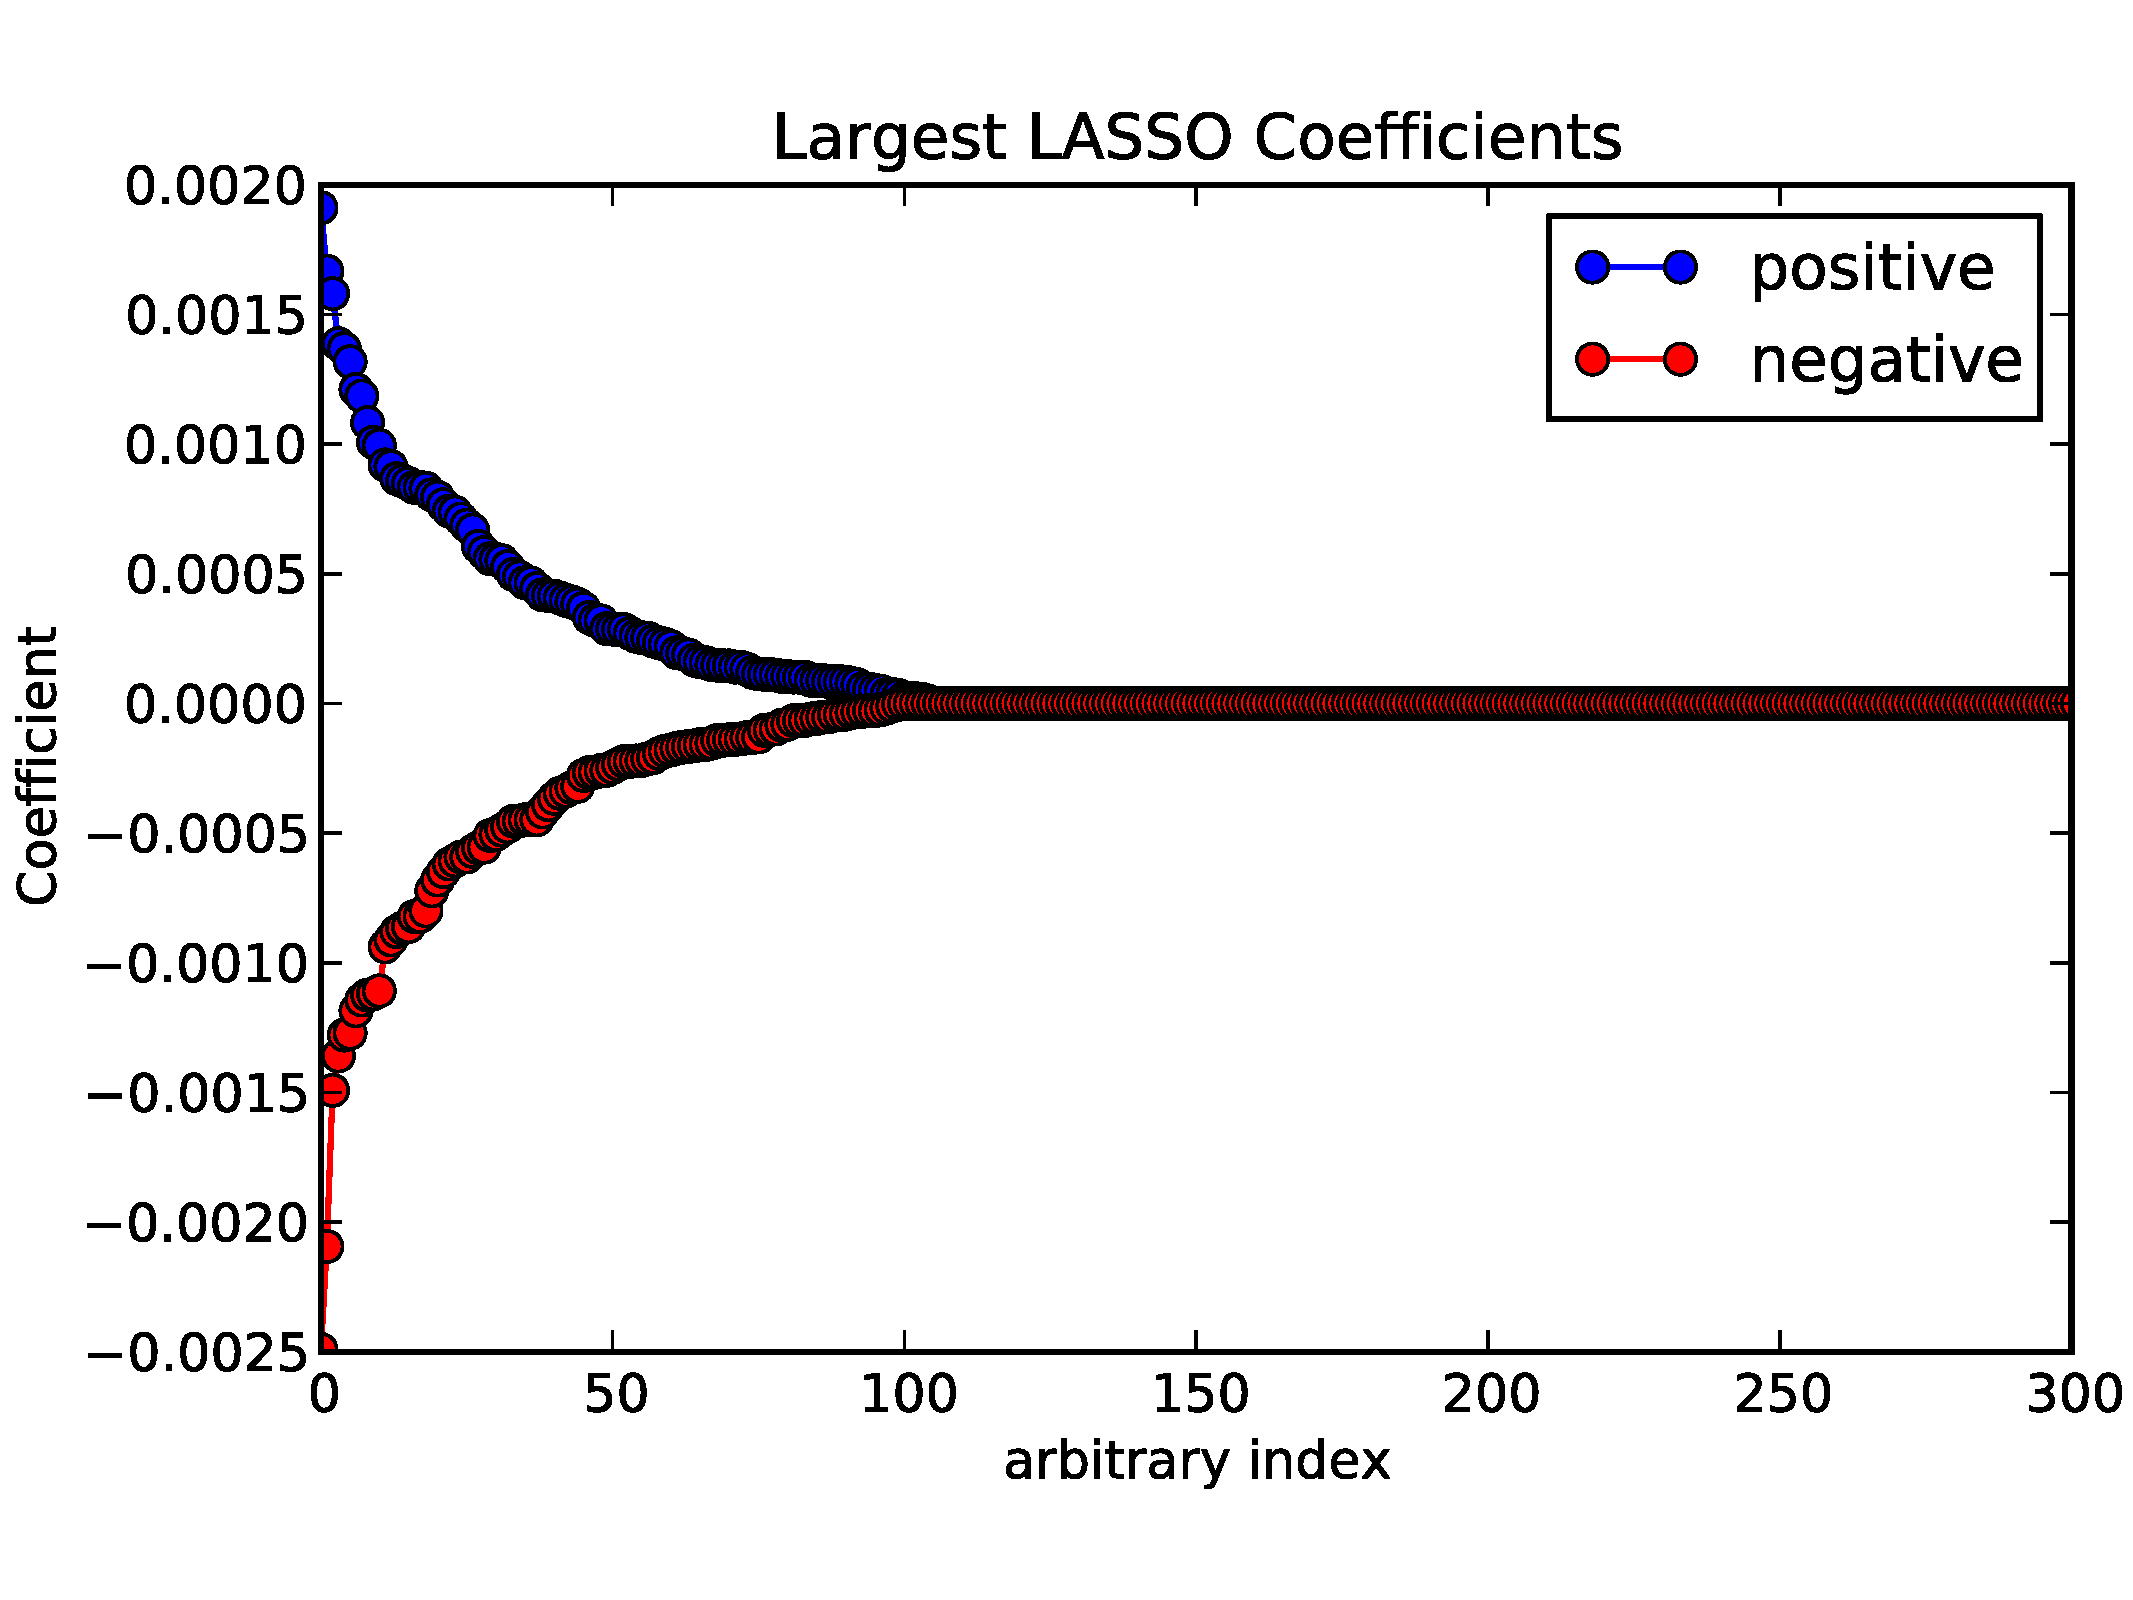
\includegraphics[width=.45\textwidth]{ag-gut-lasso-coeff.pdf}\label{fig:lasso coeff}}
  \subfigure[lasso MSE as a function of $\log\lambda$]{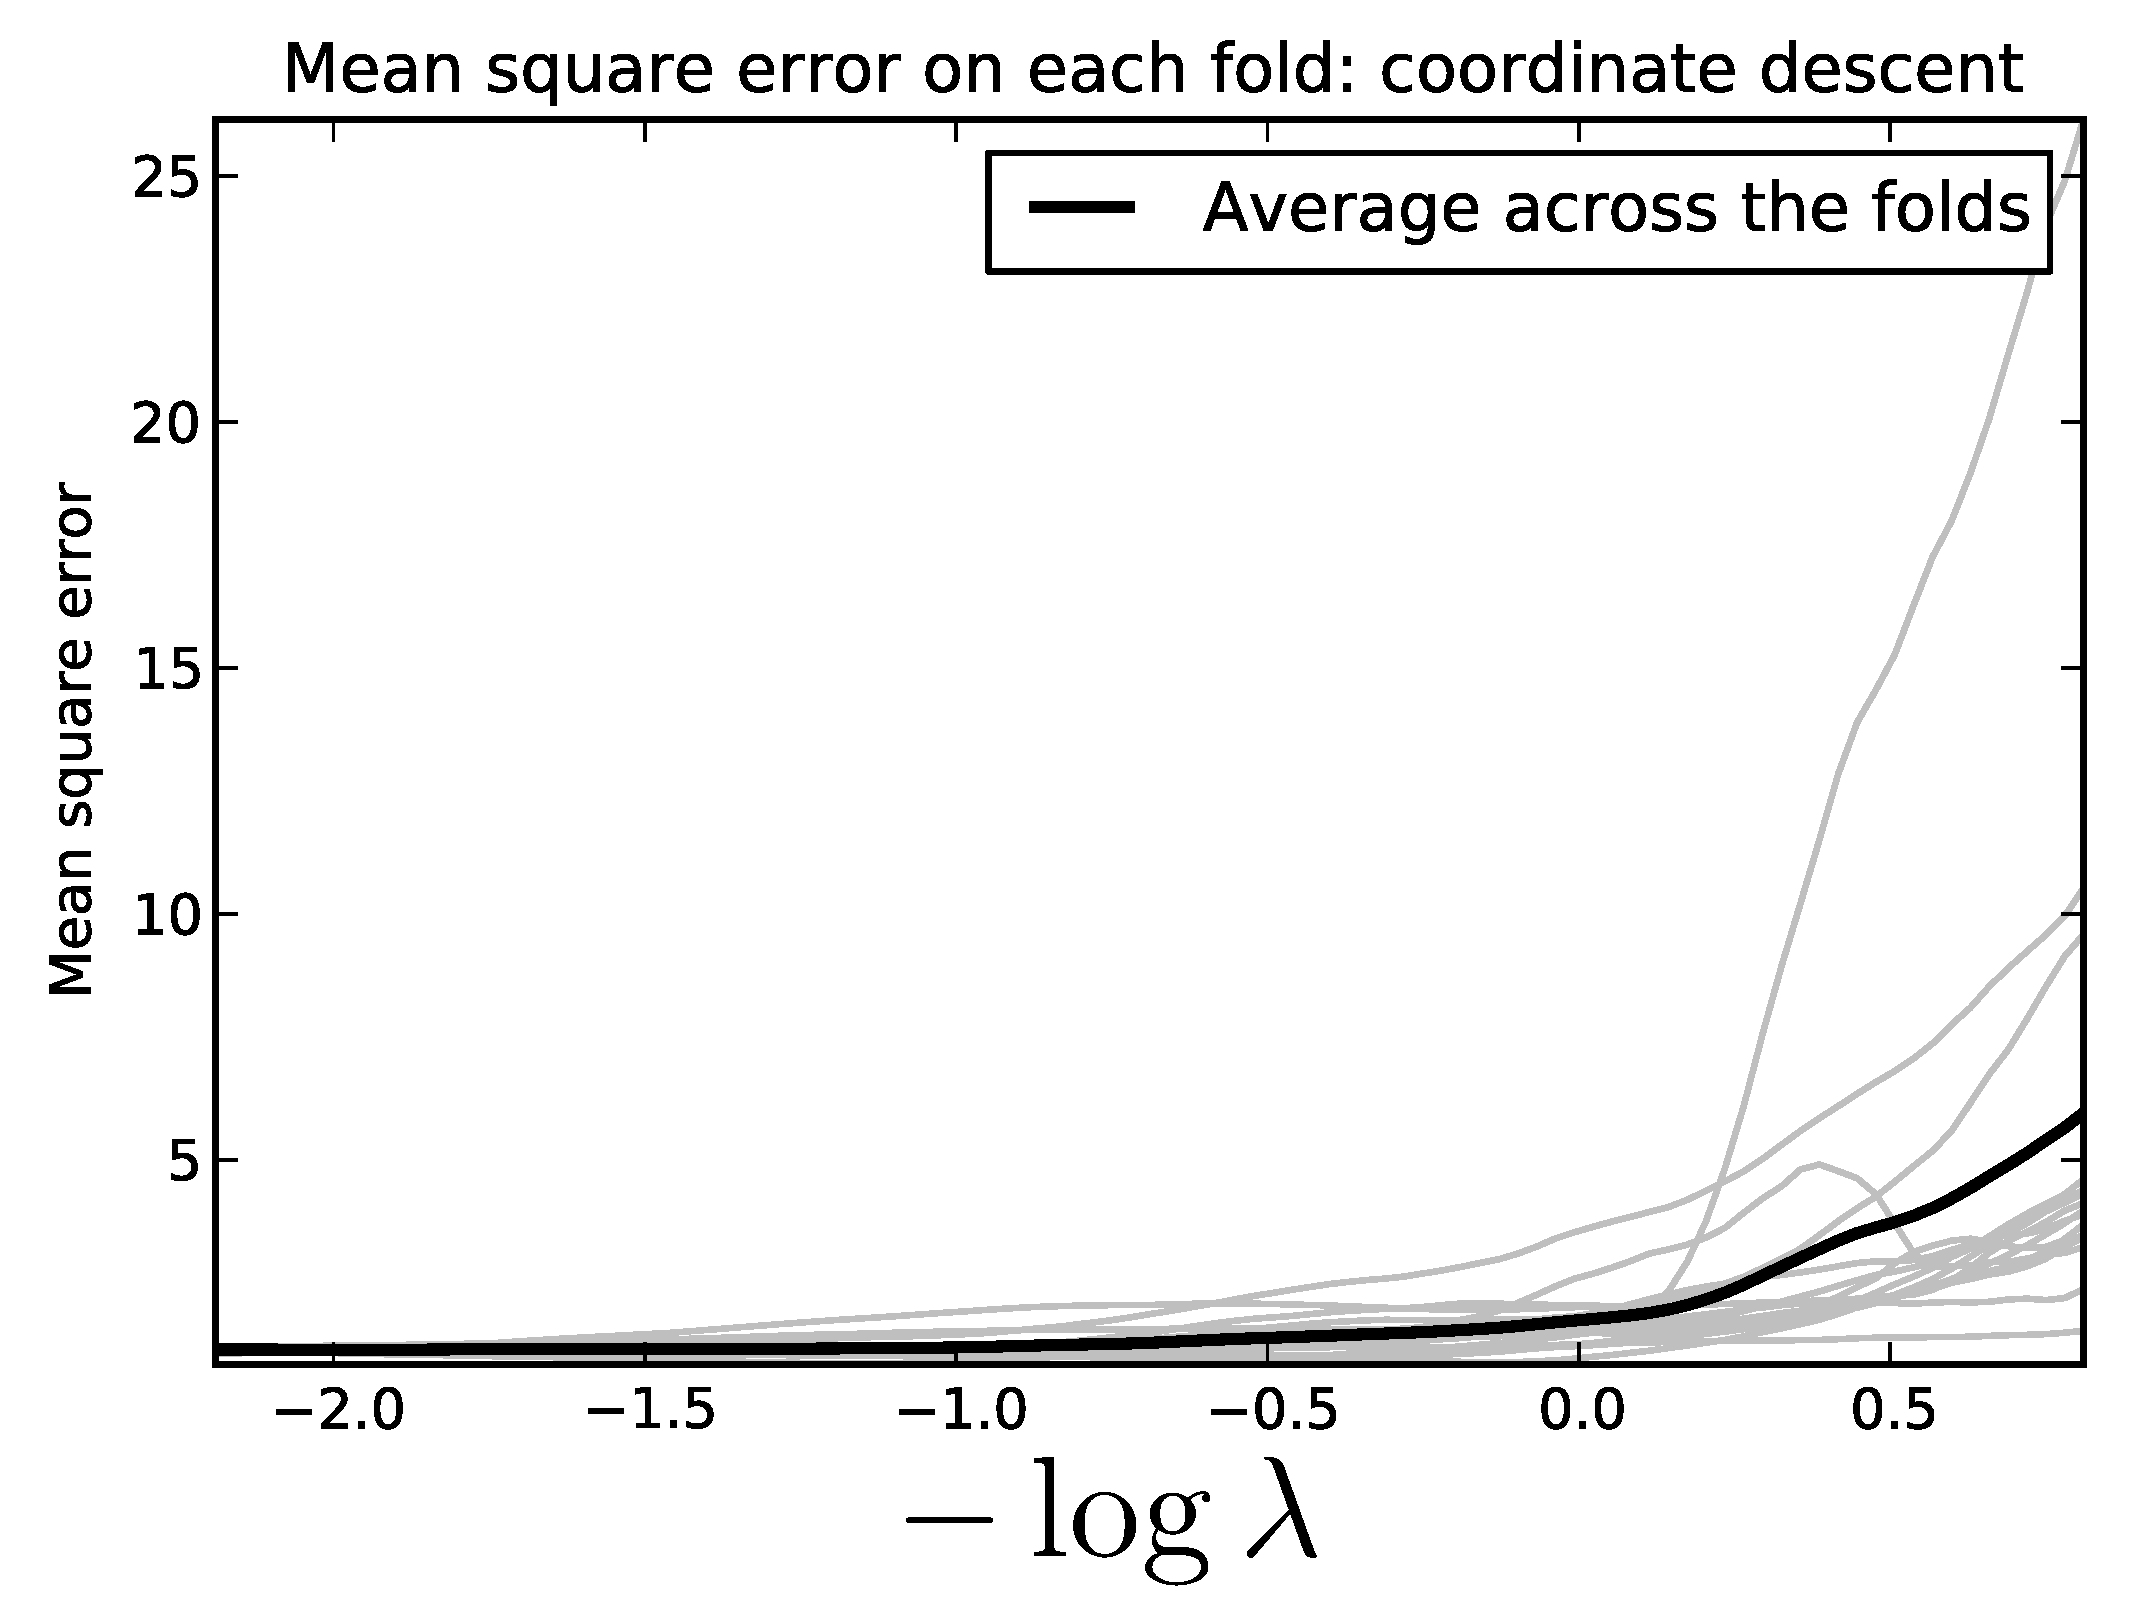
\includegraphics[width=.42\textwidth]{ag-gut-lasso-cv-mse.pdf}\label{fig:lasso mse}}
  \caption{Coefficients and the MSE of lasso applied to data from the American Gut Project.}
  \label{fig:lasso}
\end{figure*}


\subsection{Detecting Taxa Importance}
The previous section solely focused on the examining the {\em general} amount of mutual information found in sex phenotype of the American Gut Project; however, we did not examine which OTUs are being ranked as important. Below is a list of the top 10 ranked OTUs as determined by the magnitude of the weight lasso assigns to each OTU. 

\begin{mitemize}
%lasso
\item {\em Bacteria, Bacteroidetes, Bacteroidia, Bacteroidales, Bacteroidaceae, Bacteroides uniformis}
\item {\em Bacteria, Bacteroidetes, Bacteroidia, Bacteroidales, Prevotellaceae, Prevotella copri}
\item {\em Bacteria, Firmicutes, Clostridia, Clostridiales, Ruminococcaceae}
\item {\em Bacteria, Firmicutes, Erysipelotrichi, Erysipelotrichales, Erysipelotrichaceae, Eubacterium dolichum}
\item {\em Bacteria, Firmicutes, Clostridia, Clostridiales, Ruminococcaceae}
\item {\em Bacteria, Bacteroidetes, Bacteroidia, Bacteroidales, Bacteroidaceae, Bacteroides}
\item {\em Bacteria, Proteobacteria, Gammaproteobacteria, Cardiobacteriales }
\item {\em Bacteria, Cyanobacteria, Chloroplast, Streptophyta}
\item {\em Bacteria, Proteobacteria, Gammaproteobacteria, Xanthomonadales, Sinobacteraceae}
\item {\em Bacteria, Firmicutes, Clostridia, Clostridiales, Lachnospiraceae, Blautia producta}
\end{mitemize}

Furthermore, the top ten OTUs that NPFS detects as relevant are given by:
\begin{mitemize}
%npfs
\item {\em Bacteria, Bacteroidetes, Bacteroidia, Bacteroidales, Bacteroidaceae, Bacteroides}
\item {\em Bacteria, Bacteroidetes, Bacteroidia, Bacteroidales, Bacteroidaceae, Bacteroides}
\item {\em Bacteria, Firmicutes, Clostridia, Clostridiales, Lachnospiraceae, Blautia}
\item {\em Bacteria, Proteobacteria, Betaproteobacteria, Burkholderiales, Alcaligenaceae, Sutterella}
\item {\em Bacteria, Firmicutes, Clostridia, Clostridiales, Ruminococcaceae}
\item {\em Bacteria, Bacteroidetes, Bacteroidia, Bacteroidales, Bacteroidaceae, Bacteroides}
\item {\em Bacteria, Firmicutes, Clostridia, Clostridiales}
\item {\em Bacteria, Firmicutes, Clostridia, Clostridiales, Ruminococcaceae}
\item {\em Bacteria, Firmicutes, Clostridia, Clostridiales, Ruminococcaceae, Ruminococcus}
\item {\em Bacteria, Firmicutes, Clostridia, Clostridiales, Lachnospiraceae, Ruminococcus, gnavus}
\end{mitemize}
where some OTUs are repeated because repeats in the 25k+ OTUs in the original dataset. For both lasso and NPFS, we observe {\em Bacteroidetes} is commonly being detected as OTU with high differentiation between the individual's sex, which {\em Bacteroidetes} has been hypothesized to be factor between male and female guts' differences \cite{Xu2012MicoB}. 

\begin{figure}
  \centering
  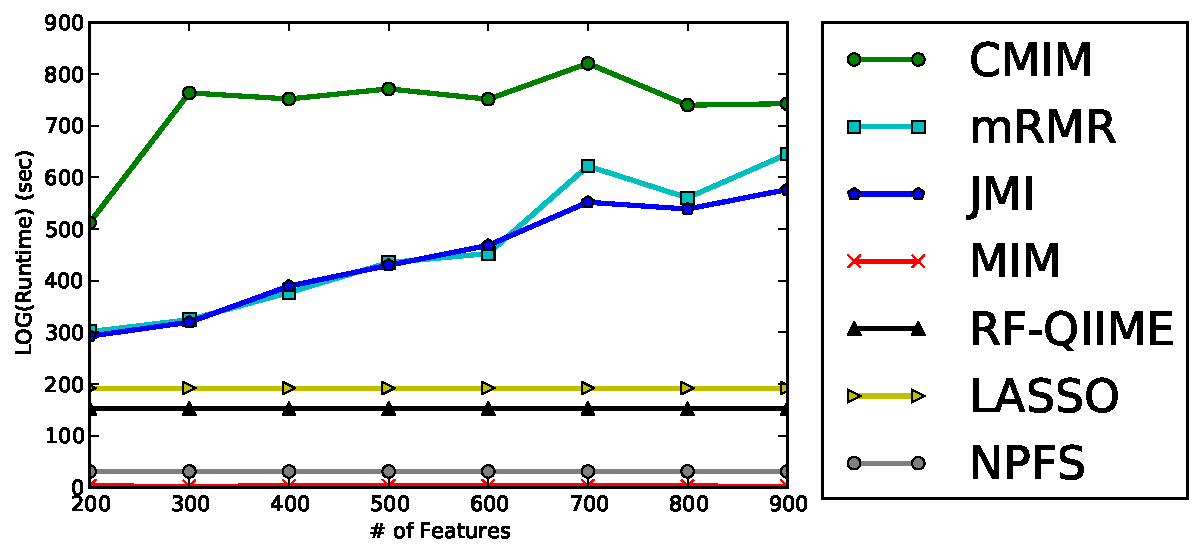
\includegraphics[width=.45\textwidth]{runtime.pdf}
  \caption{Runtimes seven algorithms that can be used for selecting important taxa. Note that times for NPFS, LASSO, and RF-QIIME are simply interpolated from 200 to 900 because they select a fixed number of taxa. }
  \label{fig:times}
\end{figure}



\subsection{Implementation Tradeoffs}

Finally, we address the time it takes to evaluate several different subset selection algorithms on Caporaso et al.'s data collected from the Earth Microbiome Project. Figure \ref{fig:times} shows the runtimes of seven subset selection algorithms as a function of the number of features that the selection algorithm chooses (note that CMIM, mRMR, JMI and MIM are implemented in the Fizzy's feature selection). Its important to note that NPFS, LASSO and RF-QIIME can either: (a) detect the number of relevant features, or (b) weight the features and allow the user to choose what weight values qualify an OTU as being important. Hence the reason NPFS, LASSO and RF-QIIME is shown as being ``fixed'' w.r.t. the number of features being selected by the algorithm.  From Figure \ref{fig:times}, we observe that MIM has the fastest runtime, which is closely followed by NPFS. NPFS has the advantage of being extremely parallelizable, which our software implementation takes advantage of. The final runtimes for lasso, random forests, and NPFS were 192.2s, 152.7s, and 30.8s, respectively. 


\section{Conclusions}
\label{sec:conc}

In this work, we evaluated embedded and filter based feature subset selection algorithms on data collected from the gut microbiome. We've shown there are very few OTUs that provide information for making these predictions using both information-theory and lasso. Furthermore, NPFS and MIM were shown to provide results from subset selection that go along with our intuition about the microbiome, while being extremely competitive in regards to runtime. NPFS's runtime can be improve further -- nearly to the runtime of MIM -- if more processor were available. This is because of NPFS's ability to be highly parallelized.  

\section{Acknowledgements}
G. Ditzler and G. Rosen are  supported by the NSF CAREER award \#0845827, NSF Award \#1120622, and the Department of Energy Award \#SC004335. 



\bibliographystyle{abbrv}
\bibliography{/Users/gditzler/Dropbox/Public/Research/Bibtex/greg_refs.bib}



\end{document}
